\chapter{Design and Specifications}
\label{chap:figtab}
\label{chap}

\section{Specifications}

 The objective of this software is to  a dynamic user interface and a functional database system. With regard to that, the specification is made up of necessary features and functionality that appear on the user interface. The following are the major specification of this software:
\begin{description}
\item[$\bullet$] User Log in
\item[$\bullet$] Data Inventory
\item[$\bullet$] Searching Inventory(SI)
\item[$\bullet$] Make Reservations
\item[$\bullet$] Cancel Reservations
\item[$\bullet$] Add data
\item[$\bullet$] Update data
\end{description}
Registered users have access to the system with unique user name, so the user interface provides a log in form on the web page where user can submit their details to be stored in the database. The user interface is able to list the inventory of data stored in the database in different categories. This is one of the main features of the user interface because it presents the content of the database. As there are data inventory on the user interface, it is necessary to have a function that allow users to search information from the inventory.  Another requirement of this software is the ability to make reservations: users are able to choose a machine from the inventory and reserve it for a fixed date and time. This requirement on the high level is meant to allow user to a specific machine for running a particular task on that machine without interruption. When a reservation made is expired, the machine that was reserved becomes free for other users. As new machines are added to the cluster, the Add-data functionality allows users to add details of those machines to the database and update the inventory. Likewise, when the user want to change a certain properties of the machines such as, memory size or disk, the Update-data functionality helps to perform this action.


\section{Design}
The main idea of the software is to solve the issue of user interface, and system management. So we have designed this software with the approach to provide functional solution to the specifications. The design structure comprises the various  segments and element of the user interface (front end) combined with the database (back end)  and the control protocols. 

\begin{figure}[h]
  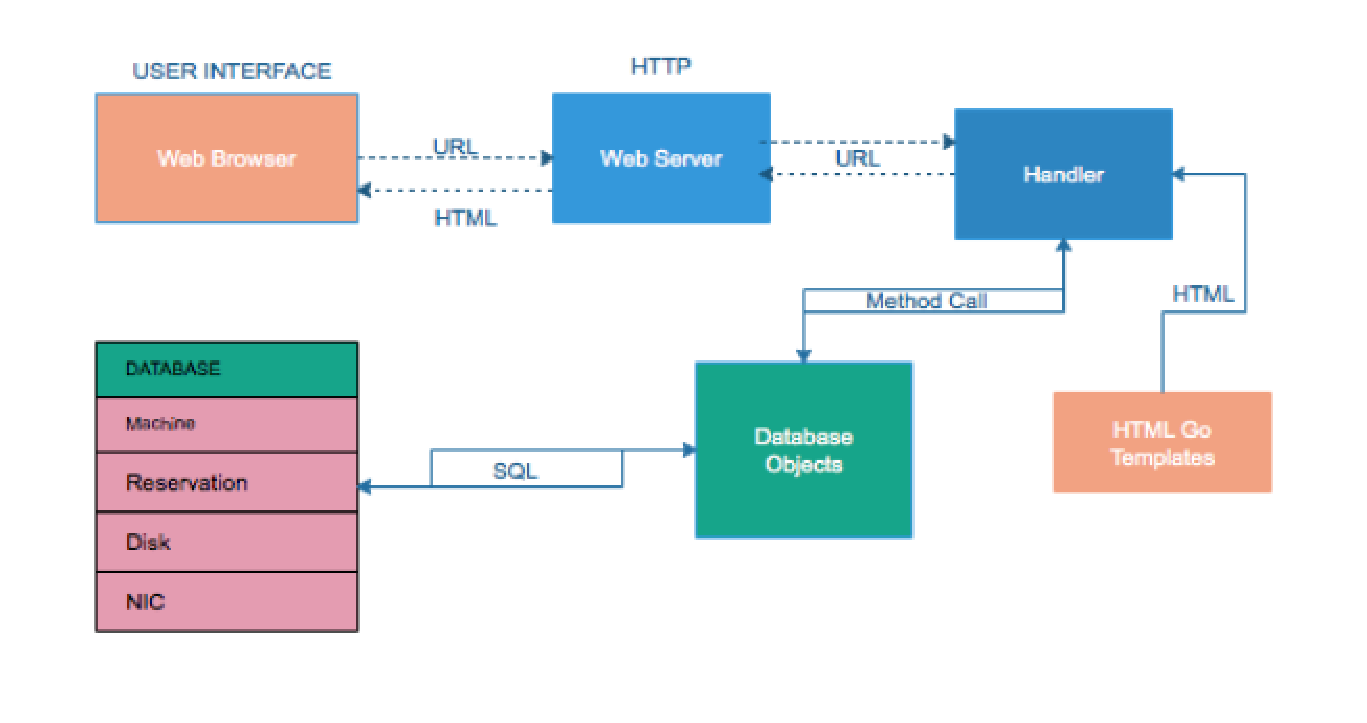
\includegraphics[width=\linewidth]{design.eps}
  \label{fig:Design of program}
  \caption{Design}
\end{figure}

We designed a web interface that provides  flexible and dynamic access to the system with interactive functionality. This web page contains inputs and output features. The reason for choosing a web page instead of other options is to provides online dynamic and simultaneous  access to the system rather than performing manual command prompts (example: checking the usage of machine, properties of machine, and status of machine ). Another reason is to have a functional real time user interface that present the activities of the Clowder. The web server is responsible for serving the web page all the resources requested by the users, and it serves as a channel between the user and the database. We designed an operational (event recording and system referencing) database that address the issue of system management. The database stores data from the web page and also retrieves data on the web page via the server. As the user log on to the their account on the web page the server will pass this information to the  database which is controlled by the main program (command protocol). The command protocols is responsible for handling the user interface activities and executing the database queries .  Below is a figure that describe the main structure of the design in terms of operation.

\subsection{User Interface}
The web interface represents the user interface (UI) where users get access to the system. It is part of the design that represents the front end of the software.The web interface elements controls the basic functionality for data input and out put. It represent each feature as mentioned in the specification. This web interface structure is designed using  HTML template as the front end and Go programming language as the back end. Below figure discribes the web interface avtivity;

\begin{figure}[h!]
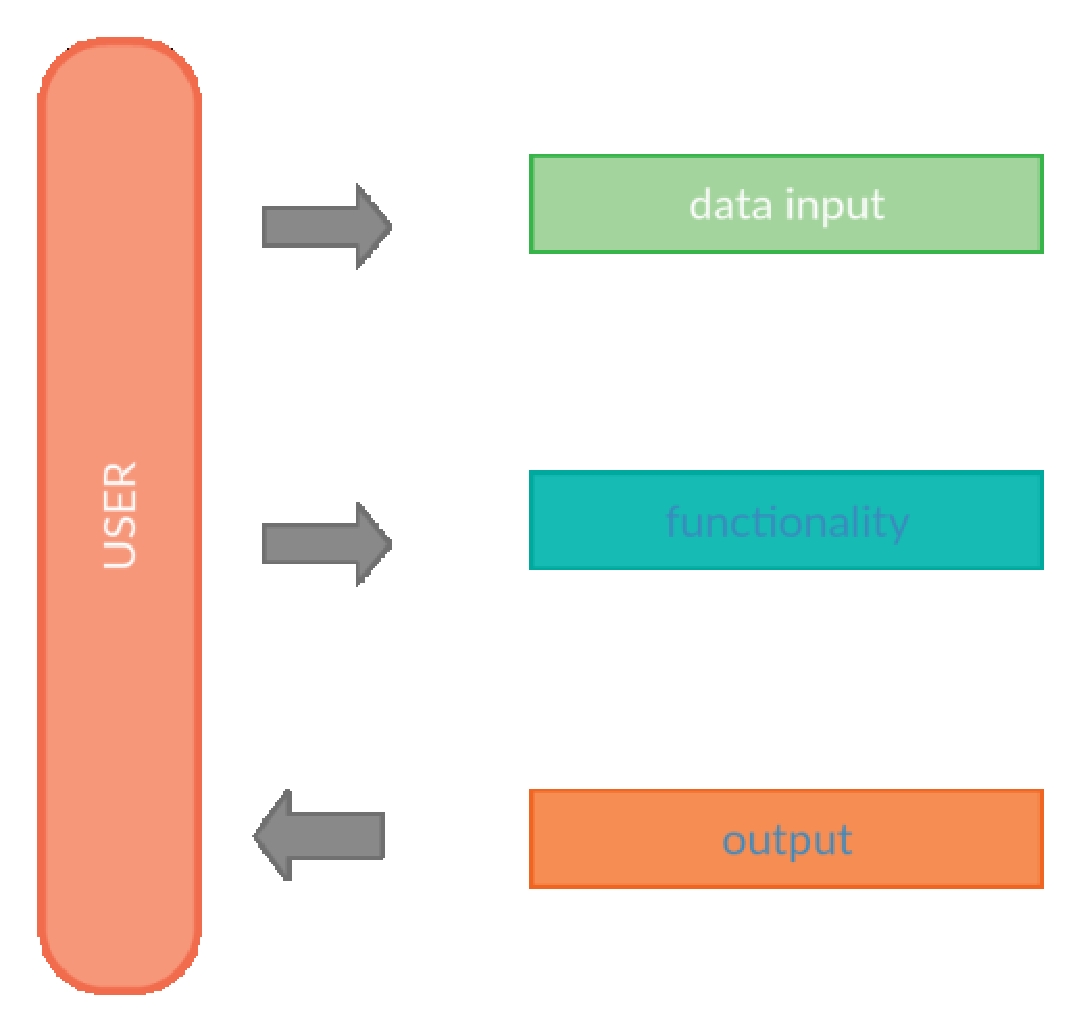
\includegraphics[width = \linewidth]{userinterface.eps}
\label{fig:Web Interface Activity} 
\caption{User Interface Description}
\end{figure}


 The web interface contains all the necessary elements required to have dynamic and flexible access to the system. These elements includes:
\begin{description}
  \item[$\bullet$] Forms
  \item[$\bullet$] Input controls
\end{description}
\subsection*{Forms}
 Forms are one the elements that provides the ability to input data to the database.The data is submitted through a HTML post request. The post forms are used for submitting data such as machines and reservations details. The form is designed with elements which includes; id and name attributes for identifying data, text fields for collecting data, select menus for selecting data options and submit button for submitting the data. When data is submitted with HTML form, the Go HTTP framework in the web server call the Go function handler to process and parse this data to the database.  After the data (example: a database query) is processed, the Go program generates an HTML page (such as machines inventory), which the server returns to the web interface. In this system design, the forms are used for creating new machines, disks, NICs and making reservation. 
 
\subsection*{Input Controls}
The input control in this web interface provides the necessary components that supports the functionality of the software. There is array of HTML input control, but we have chosen a few that satisfy our specifications. These input controls includes text field, buttons, date fields, drop down list and list box. They are used for both input and output functions like listing the inventory, inserting texts, to update data, to send queries, viewing selection options and searching inventory. These controls are designed with HTML tags and HTML template.

\subsection{Server}
The server is responsible for parsing all request from the web interface to the database and command protocol. When request is made on the web interface (for instance available machine on database), the server calls the  specific function of command protocol to handle this request by providing the necessary resources. Likewise the server interchange communication between the user interface and the database system for executions and requests. 

\begin{figure}[h!]
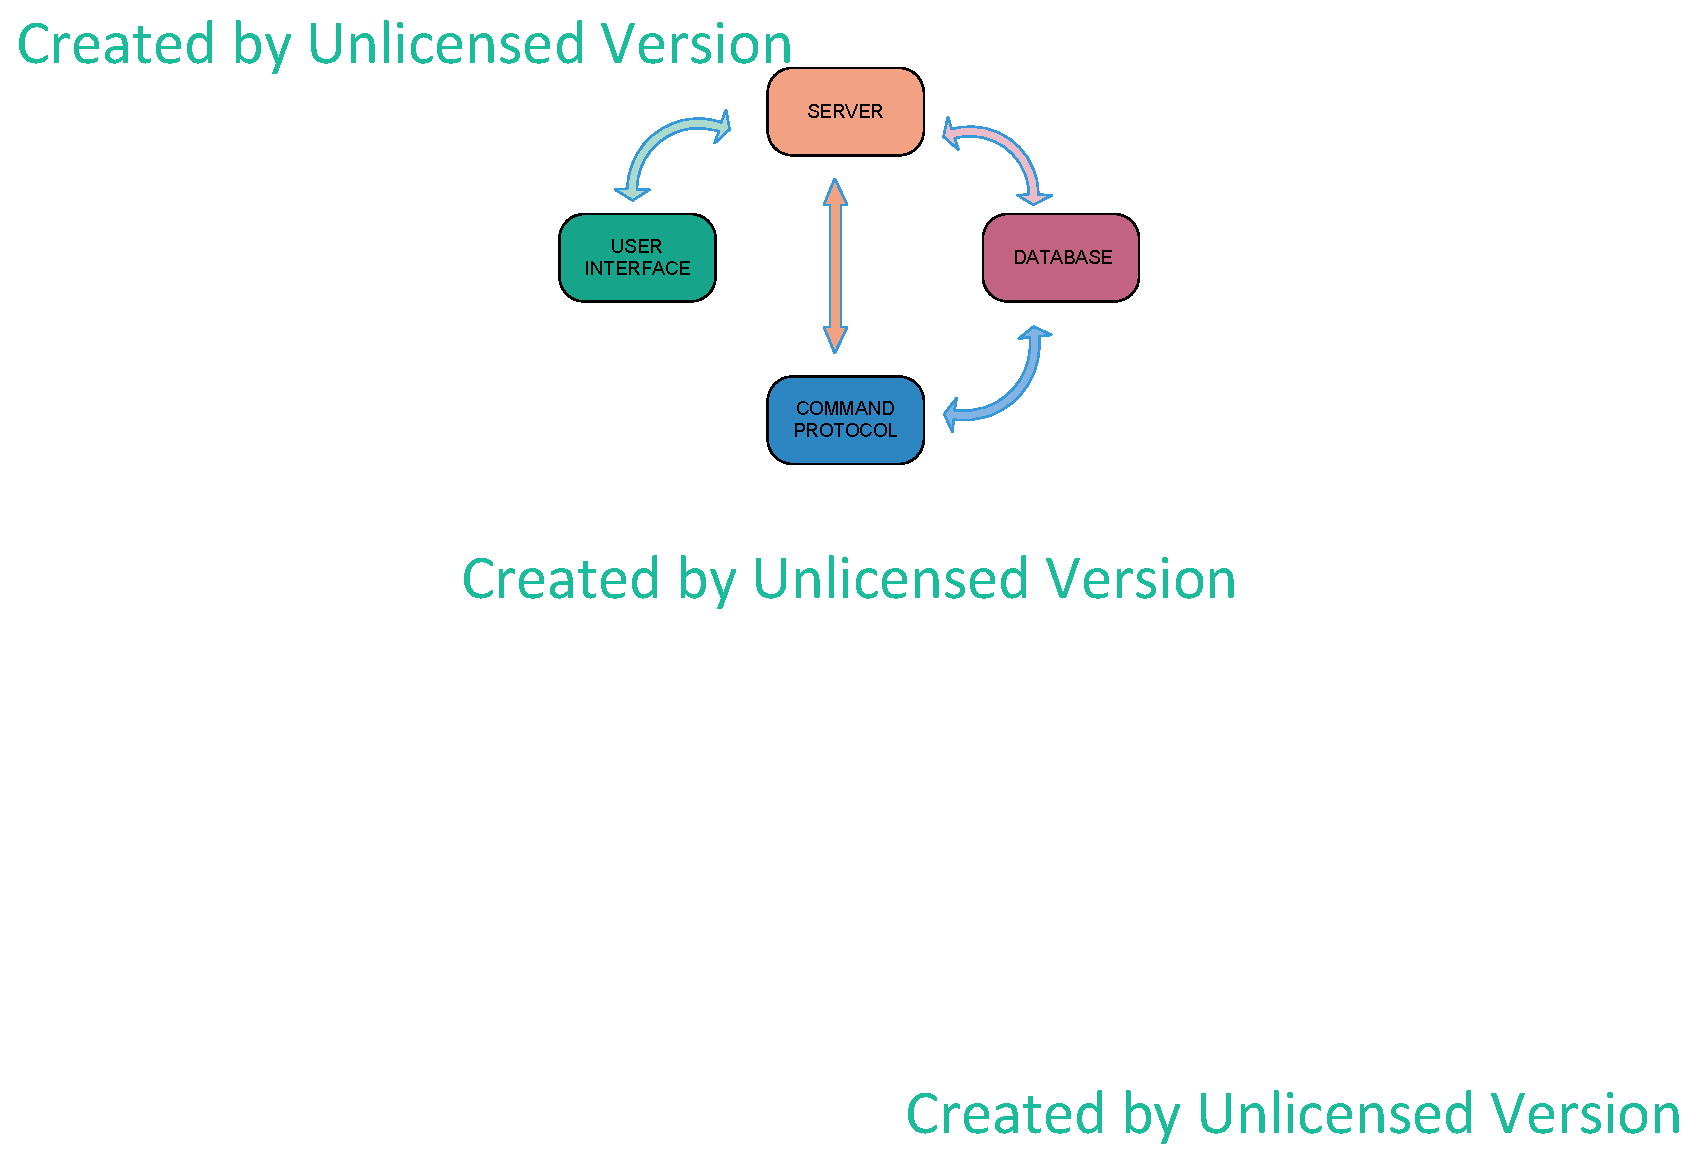
\includegraphics[width = \linewidth]{design1.eps}
\label{fig:Description of Server Activity} 
\caption{Server Activity Description}
\end{figure}

\subsection{Database}
The database is another major component of this system, because it is provides storage and resource for the system. The data includes reservation records, machine details, disks, and NICs information. The database is designed with SQLite model using Go programming language as the back end tech. SQlite was used here because its a fast open source SQL engine. We created a functional database system that suites the specification of the software. 
The database scheme contains tables of machines, user record, reservation, NICs (network interface cards) and disks.  One of the function of the software is the ability to make reservations.  Below show a typical model of the database design.

 \begin{figure}[h!]
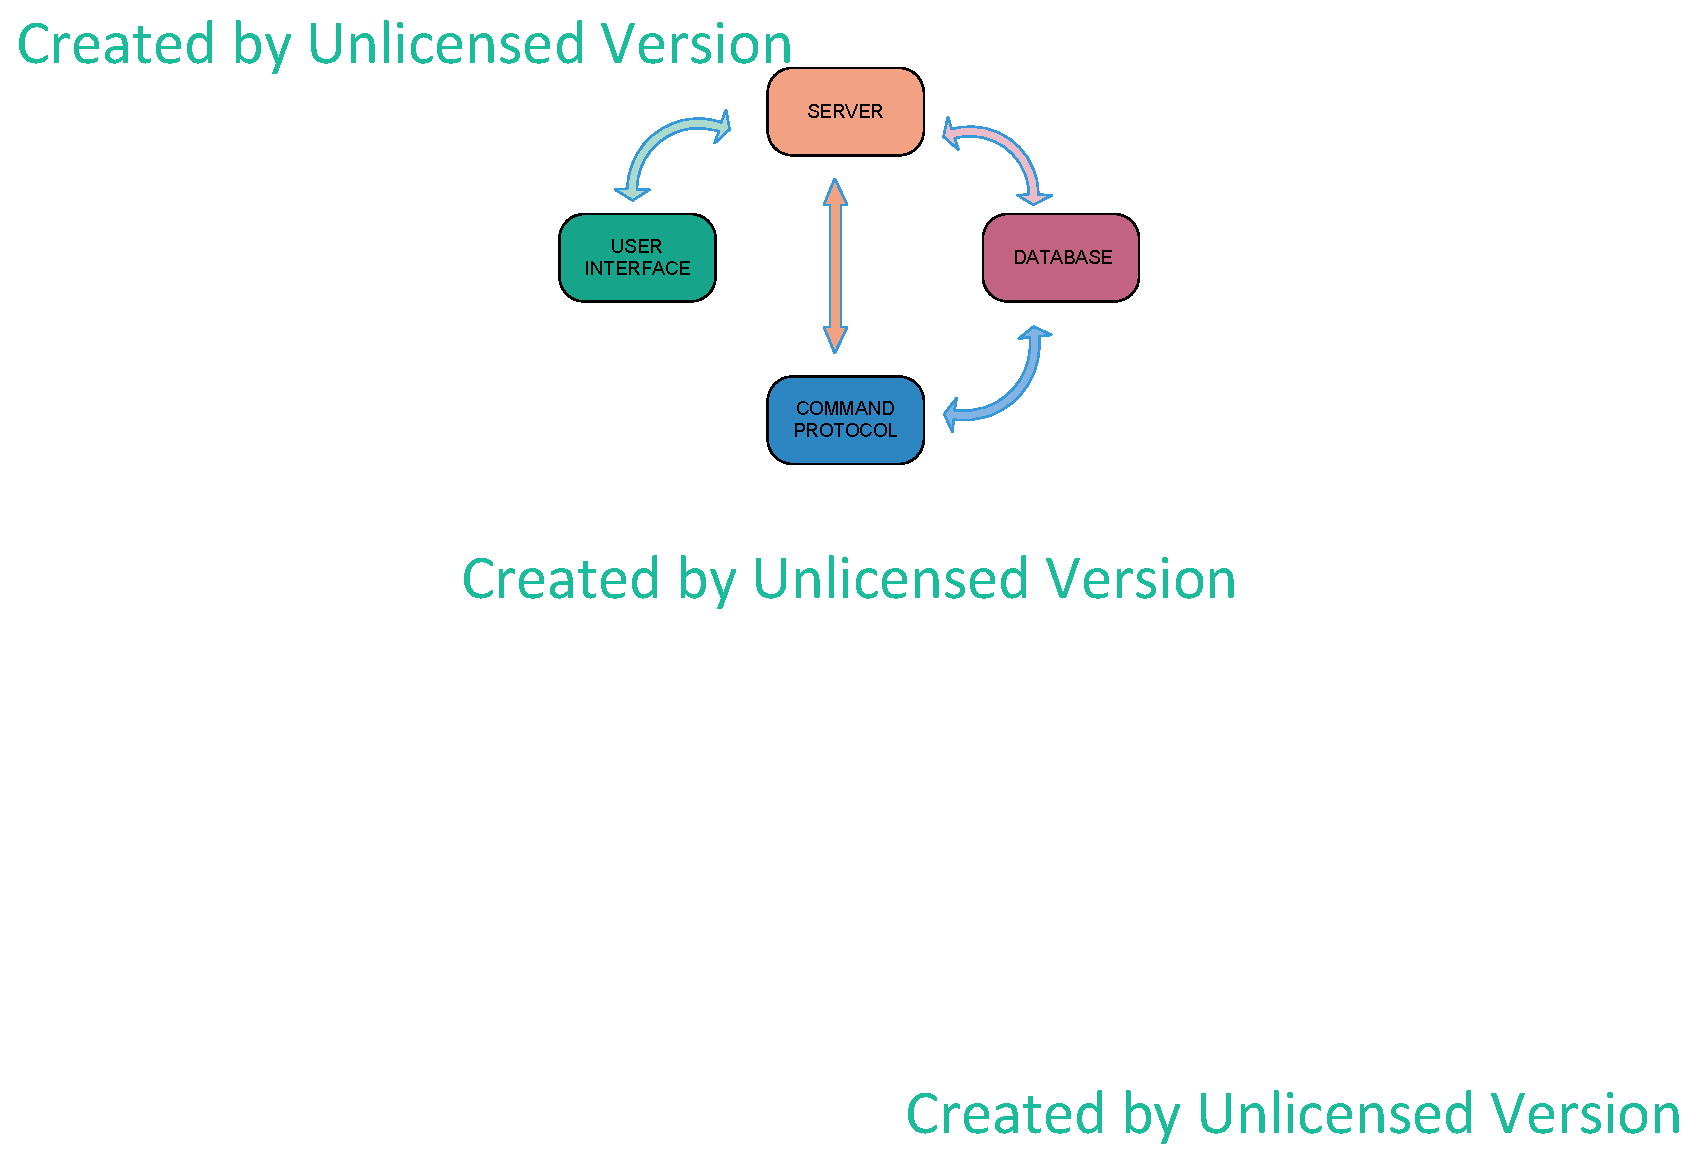
\includegraphics[width = \linewidth]{design1.eps}
\label{fig:Database Schema} 
\caption{Database design}
\end{figure}

\subsection{Command protocols}

\subsection{Design Data Flow}



